\section{Methodology}

\subsection{Hardware}
The experiments conducted in this report were performed on a computer with the following specifications:
\begin{itemize}
	\item CPU: i5-2500 (4 cores @ 3.3-3.7	GHz)
	\item RAM: 8 GB DDR3
	\item OS:  Ubuntu 15.04
\end{itemize}

\subsection{Introductory Experiments}
To foster familiarity with Octave, a task was issued that involved generating a .wav file with a given method, and then creating one for comparison. The difference between the two functions being that the first one relies on a single call to rand() to generate multiple values, while the new method makes a call to rand() for each value in turn. A sample rate of 8000Hz was used, to decrease computation time. 


The code for the custom implementation is shown below:

\begin{Matlab}
function whiten = createwhiten(time)
  sample_rate = 8000;
  whiten = zeros(time*sample_rate,1);
  samples = time*sample_rate
  for i = 1:samples
    whiten(i) = rand();
  end
  
  whiten = whiten*2-1; %fit into .wav bounds
end
\end{Matlab}

It is unlikely that the custom implementation will be able to perform better than the likely highly optimized native function.

\subsection{Custom Correlation Implementation}
The source code for the bespoke correlation solution is shown below. I would expect this code to run more quickly than the native implementation at least for some cases, as it relies on basic arithmetic principles, and offers no additional functionality.

\begin{Matlab}
function r = mycorr(x,y)
	% readability >> succinctness
	sx  = sum(x);
	sy  = sum(y);
	sxy = sum(x.*y);    % elementwise multiplication
	sx2 = sum(x.^2);    % elementwise squares
	sy2 = sum(y.^2);
	n   = max(size(x)); % just in case we get some column/row vector mixups
	num = sxy - sx*sy/n;
	den = sqrt((sx2-(sx.^2)/n)*(sy2-(sy.^2)/n));
	r = -2; % default, in case correlation could not be performed
	if(den != 0)
		r = num/den;
	end
end
\end{Matlab}

\subsection{Comparing Signals Shifted in Time}

Firstly, a signal must be generated, and then compared against a shifted version of itself. This can easily be done by generating a signal and then using a small 'window' of the signal compared to a window shifted slightly to either side, i.e. if the signal x is comprised of 100 samples, one signal could be x[1:50] and the shifted version 20 samples ahead, at x[21:70]. For all instances, I used a window size of 50 samples.

The signals generated were sine waves, at frequencies of 1rad/s, 2rad/s, and 10rad/s. All of the signals generated range from -pi to pi. 100, 1000, and 10000 samples were used for each frequency.  The choice of windows are [1:50] (the first 50 samples of the signal), [2:51] (a shift by 1), and [11:61] (a shift by 10). Figure~\ref{fig:absvals} shows the absolute value of the differences between shifted signals at different sample rates, indicating that higher sample rates have smaller differences between nearby samples than lower sample rates.

These values were chosen to cover a wide range of signals, and to avoid jumping to conclusions.

It is hypothesised in this report that correlating a sinusoid with a time-shifted version will have the following effect on the Pearson's Correlation Coefficient:

\begin{itemize}
	\item Sinusoids are periodic, so shifting by one period will give the same correlation value
	\item Sinusoids are odd, so after half a period, the correlation will be at a minimum. It should be that r=-1 at this point, as the signals are inverses.
	\item The correlation coefficient will smoothly vary between 1 and -1 as the signal is shifted.
	\item Higher sample rate signals will be less susceptible to sample-based shifts but equally susceptible to time-based shifts.
\end{itemize}

The correlation between each signal was calculated using the native corr function as follows:

\begin{Matlab}
a = linspace(-pi,pi,100); %100 samples
x1  = sin(a*1); %frequency of 1rad/s
w1 = 1:50;
w2 = 2:51;
r = corr(x1(w1),x1(w2));
disp(r);
\end{Matlab}



\begin{figure}
\centering
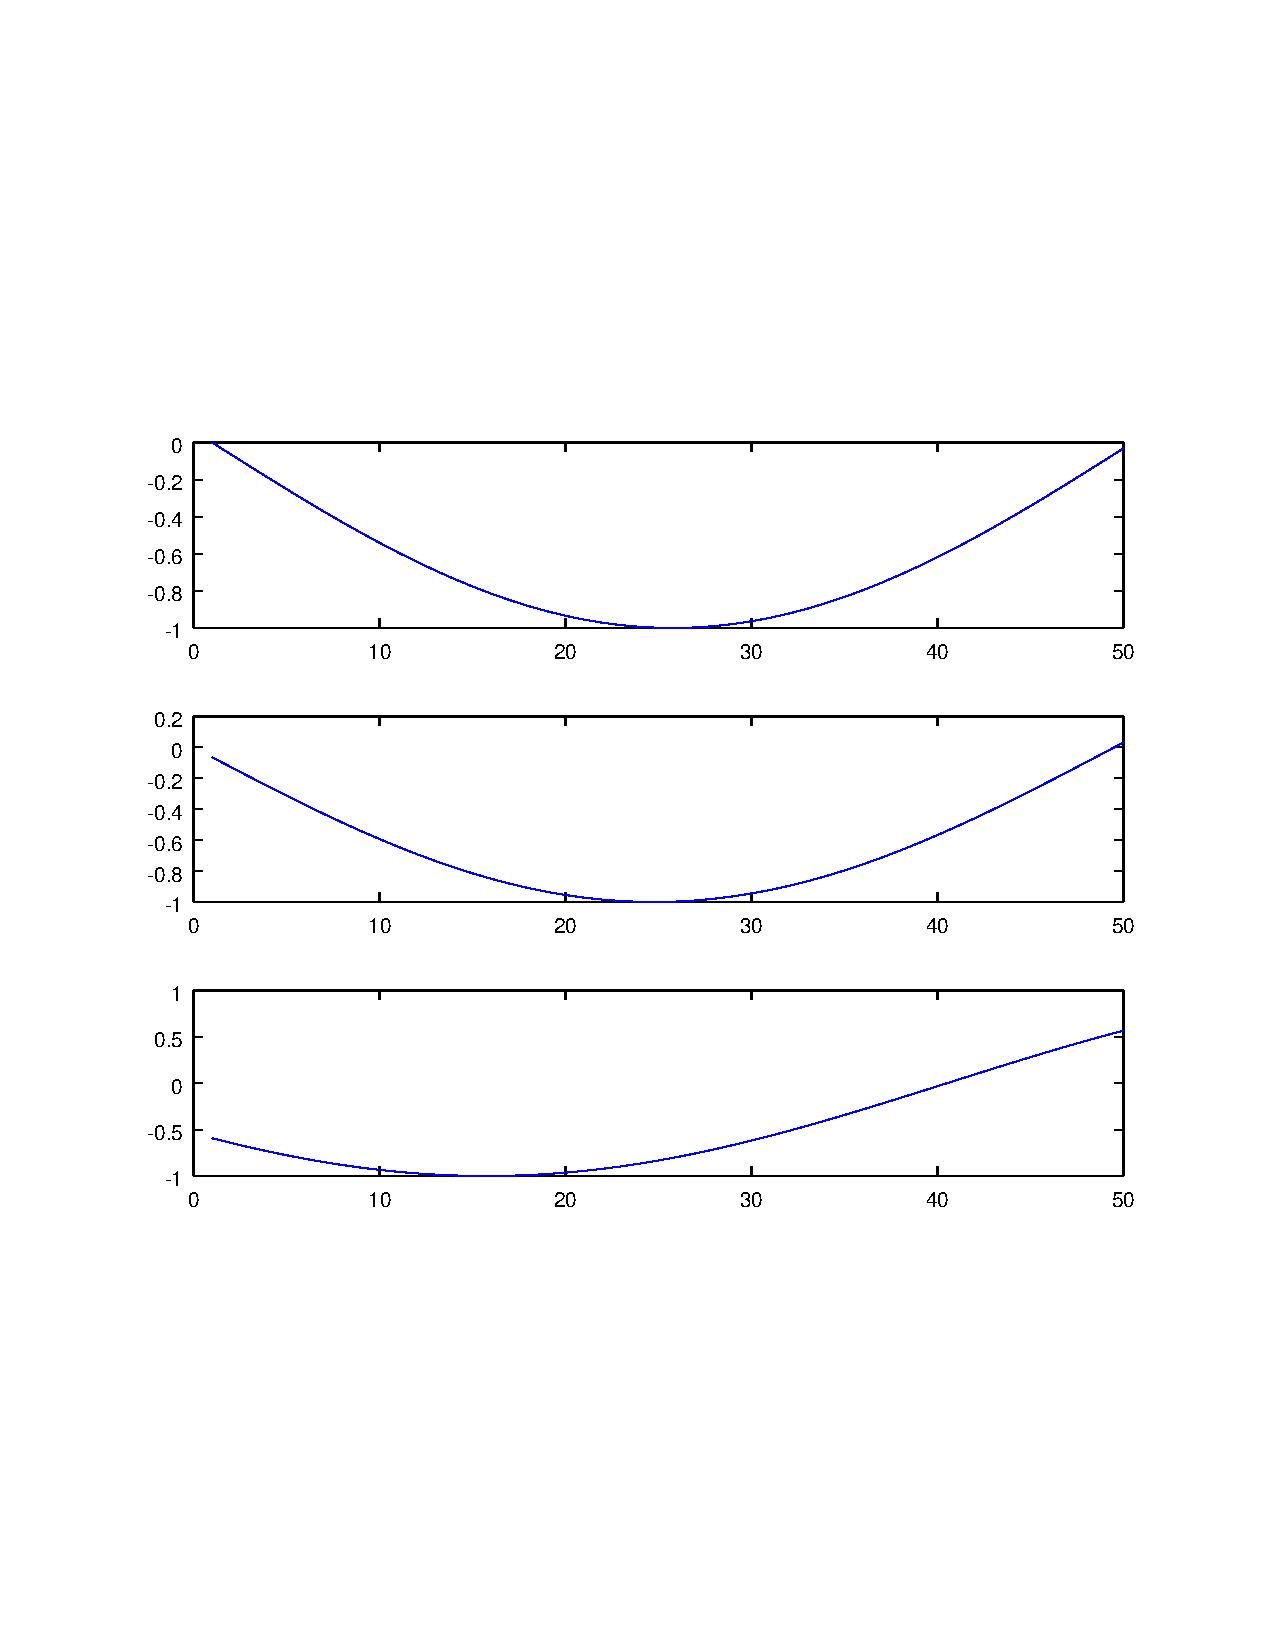
\includegraphics[scale=0.4]{Figures/lofreq}
\caption{Different windows of the same signal}
\label{fig:windowslo100}



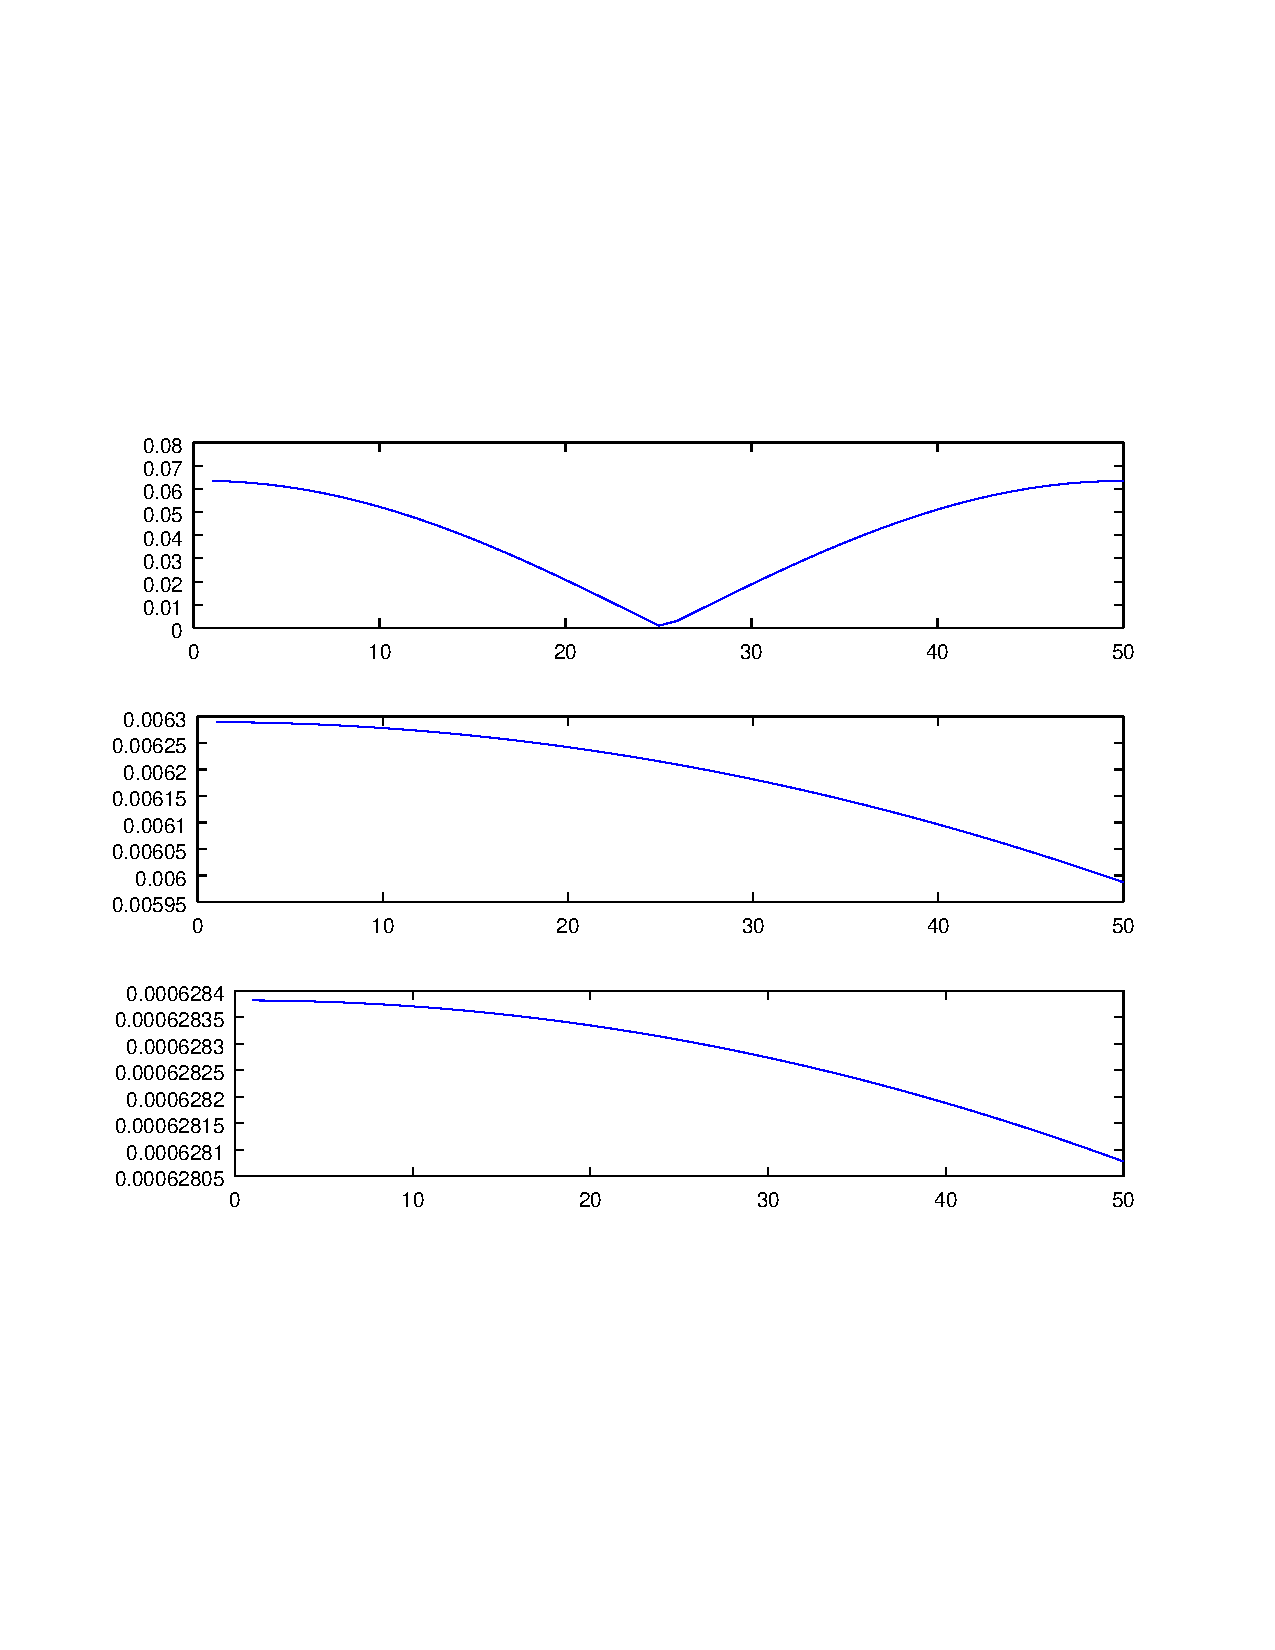
\includegraphics[scale=0.4]{Figures/absvals}
\caption{Absolute differences between a signal and shifted counterpart, according to sample rate}
\label{fig:absvals}
\end{figure}
